\section{Levels of recursion and limits on human reasoning}
\label{sec:levels}

In our next set of experiments, \exptrefrange{exp:levels-level}{exp:levels-oddman}, we probed limits on the kind of inferences we could measure in our reference game paradigm. In all of these experiments, we also conducted parallel experiments measuring prior expectations using the methods described in \secref{sec:priors}, but we largely omit discussion of these data until \secref{sec:models}. 


 \begin{figure}[t]
  \centering
  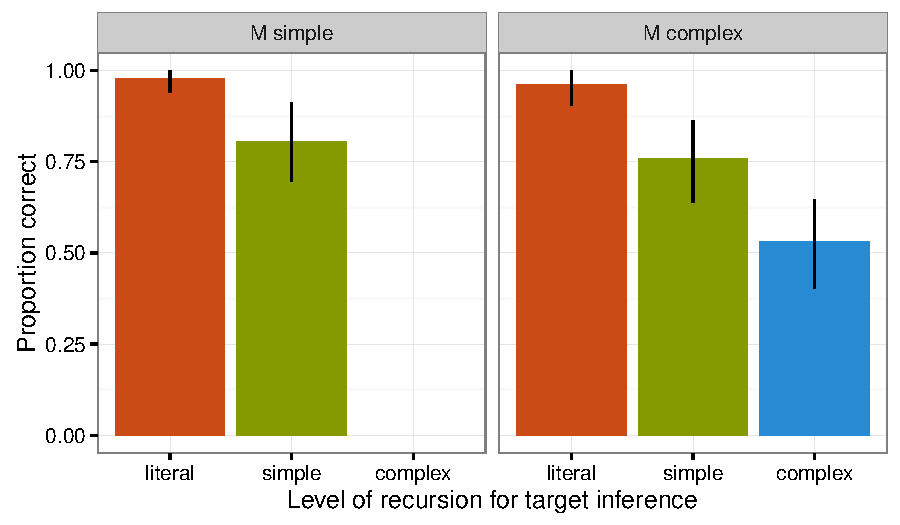
\includegraphics[width=4in]{../plots/3-levels-levels.pdf}\\ 
  A) 
\includegraphics[width=3in]{figures/hatglasses.pdf}\\
  B) 
\includegraphics[width=3in]{figures/levels-levels-stim.pdf}
  \caption{\label{fig:levels-level} Data from \exptref{exp:levels-level}, plotted by display (A being simple, B being complex) and inference level (see text).}
\end{figure}


In our first experiment, \exptref{exp:levels-level}, we attempted to measure patterns of inference in more complex reference games. Following \citeA{stiller2011} and \citeA{degen2012}, we created a matrix that required a deeper level of reasoning than our previous experiments. In particular, we compared our standard reference game (shown again for reference in Figure \ref{fig:levels-level}A) with a more complex game (Figure \ref{fig:levels-level}B):


\begin{equation}
\left[
    \begin{array}{ccc}
      0 & 0 & 1 \\
      0 & 1 & 1\\
      1 & 1 & 0 
    \end{array} 
  \right]
\end{equation}

\noindent In RSA-style models, the level of recursion $n$ describes the number of iterations of speaker-listener computation that are performed. Here we impose this notation on individual inferences and whole matrices. We refer to a ``level 1'' inference as one that an RSA agent with $n=1$ can solve (e.g., the designated target has the highest probability of the possible choices). By analogy, then, a ``level 1'' matrix stimulus is one for which all possible inferences can be answered correctly at greater than chance levels by an RSA agent with $n=1$. 

In \exptref{exp:levels-level}, we used the stimulus in Figure \ref{fig:levels-level}A to measure inferences about the pragmatic target (as above, a level 1 inference) and the target with the unique feature (e.g. choosing the hat with the word ``hat''; a level 0 inference). We also used the stimuluis in Figure \ref{fig:levels-level}B to measure a level 1 pragmatic inference (the target for this inference was the face with a mustache but no glasses, for the utterance ``mustache''). The main contribution of this experiment, however, was our test of a level 2 inference (``glasses,'' with the presumptive target the face with glasses and mustache, not glasses and hat). This inference depends on having reasoned that while both of the targets have another possible descriptor, for one of those targets, the second descriptor is unique, whereas for the other the second descriptor is also non-unique. 

As shown in Figure \ref{fig:levels-level}, judgments in the Level 1 inference remained very close to 75\%, regardless of display (the level observed across many of our other experiments). Level 0 inferences were of course at ceiling. In contrast, Level 2 inferences were at chance (53\%). The prior for this target was lower than the prior for the logical distractor image, however (23\% vs 39\%). Thus, it may be the case that participants make this inference but it is partially or fully cancelled out by an expectation against it (see Figure 1 of Frank \& Goodman, 2012, for a potential example of this kind of cancelation). 

 \begin{figure}[t]
  \centering
  
\includegraphics[width=4in]{figures/levels-twins-stim.pdf}
  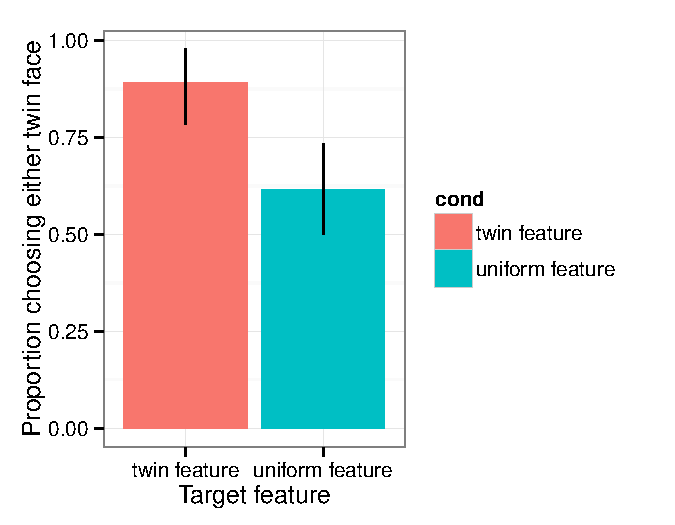
\includegraphics[width=4in]{../plots/3-levels-twins.pdf}
  \caption{\label{fig:levels-twins} Data from \exptref{exp:levels-twins}, along with the display used for this experiment.}
\end{figure}

\exptref{expt:levels-twins} further considered the scope of the inferences that participants would make by examining displays like the one shown in Figure \ref{fig:levels-twins}, top:

\begin{equation}
\left[
    \begin{array}{ccc}
      0 & 1 & 1 \\
      1 & 0 & 0\\
      1 & 1 & 1 
    \end{array} 
  \right]
\end{equation}

\noindent These displays had a uniform feature and another feature that was shared by two of the three objects. Intuitively, naming the unique feature (``glasses'') should reference the object with it. But the predictions for the other features are perhaps less clear. Should the uniform feature also resolve to the unique object (e.g. ``mustache'' means {\sc mustache+glasses})? And should the duplicated feature resolve to the duplicated objects, or to the non-duplicated object, violating the literal semantics? 

Findings, shown in Figure \ref{fig:levels-oddman}, suggest that referencing the twin feature ({\sc hat}) led to a high degree of choice of one of the duplicated referents; choice of the uniform feature ({\sc mustache}) led to more choices of the unique object. Inferences about ``mustache,'' the uniform feature'' led to a standard level 1 implicature; inferences about the ``twin'' feature provided little evidence that participants violated the literal semantics of the ambiguous predicate. 

 \begin{figure}[t]
  \centering
  
\includegraphics[width=4in]{figures/levels-oddman-stim.pdf}
  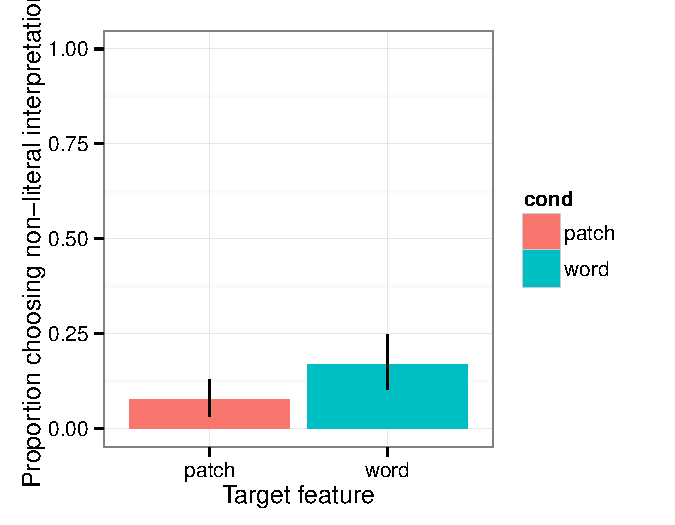
\includegraphics[width=4in]{../plots/3-levels-oddman.pdf}

  \caption{\label{fig:levels-oddman} Data from \exptref{exp:levels-oddman}, along with the display used for this experiment.}
\end{figure}

\exptref{exp:levels-oddman} further considered whether participants would reach communicative equilibria that were at odds with those implied by the literal semantics of the words the speaker used, in cases where the matrix was systematically and frustratingly ambiguous. To address this question, we used a display like the one in Figure \ref{fig:levels-oddman}, top:

\begin{equation}
\left[
    \begin{array}{ccc}
      1 & 1 & 0 \\
      1 & 0 & 1\\
      0 & 1 & 1 
    \end{array} 
  \right]
\end{equation}

\noindent Although every feature was ambiguous, a potential equilibrium would be the use of a particular feature to describe the target \emph{without} that feature. For example, here ``hat'' could refer to the face without a hat; ``glasses'' to the face without glasses; etc. But by and large, participants did not converge on this equilibrium and instead were content to choose between the two ambiguous referents. 

A second condition examined whether participants would be more or less likely to abandon the signal if it were an unconventional signal rather than a word with conventional semantics. In this condition, we recolored the features of each object (e.g., the hat and glasses) so that each had its own unique color. Bob then communicated by showing a color patch corresponding to the matching feature. Contra our initial prediction, participants stuck \emph{more} closely to the match between color patches and particular features, choosing the ``odd man out'' at very low rates. This condition suggests that it may be a feature of reasoning in these signaling games (rather than of words per se) that keeps participants from abandoning the literal semantics of the particular signals the communicator uses.

In sum, these experiments suggest that evidence for level 1 inferences was robust across a variety of displays, for example in the new matrix types show in \exptrefrange{exp:levels-level}{exp:levels-twins}). But we saw very little evidence that, in a one-shot game of the sort studied here, we would see participants abandoning the literal semantics of the words that were used. 

%%% Local Variables: 
%%% TeX-master: "pragmods"
%%% End:
